%===============================================================
\chapter{Our Games and Commercialization Support Options}
%===============================================================

\begin{chapterabstract}	
    FIT CTU offers a robust Informatics program with a specialization in computer graphics, combining theoretical foundations with hands-on coursework in areas such as programming, visualization, and user interface design. The faculty regularly organizes events like GameJams and supports a range of student-driven game projects, resulting in a diverse portfolio of innovative games. While students benefit from university-wide initiatives, incubators, and career development programs that help translate creative projects into viable ventures, entrepreneurial support is not directly embedded within FIT CTU and no options are specialized for game developers. The chapter details the game development education available at FIT CTU, showcases notable student projects, and outlines the ecosystem of events and support services that nurture both technical and entrepreneurial skills.
\end{chapterabstract}

Game development is an integral part of FIT CTU’s academic and extracurricular offerings. The Informatics programme, with its computer graphics specialization, provides students with a thorough foundation in both the theory and practice of game creation. As part of our effort to strengthen the support provided and improve the local entrepreneurial ecosystem, it is essential to understand the current opportunities available for creative development and commercialization within FIT CTU.

%===============================================================
\section{Game Development at FIT CTU}
The Faculty of Information Technology at the Czech Technical University (FIT CTU) offers a range of courses and events dedicated to game development. Currently, the faculty offers a single study programme - Informatics - which includes several specializations. Of particular relevance is the computer graphics specialization, which combines theoretical foundations with practical experience. Core theoretical courses include Computer Graphics Programming, Modern Visualisation Technologies, and Machine Vision and Image Processing, while more hands-on experience is provided through courses such as Multimedia and Graphics Applications, Programming of Graphic Applications, and User Interface Design.

In addition, FIT CTU is preparing a new study programme - Applied Informatics - which will introduce three new specializations: Game Development, Graphics, and Computer Vision. This programme is expected to offer a stronger emphasis on practical experience and expand the number of study places available in game-related fields. As a result, a broader range of student-developed games is anticipated - many of which could benefit from structured entrepreneurial support.

Game development is also integrated into other CTU courses, such as Team Software Project, where students have the option to work on game-rated projects as part of their coursework.

The FIT CTU GameJam is another key event fostering game development. Held over an extended weekend, this 48-hour challenge tasks students with creating a computer game from scratch. Participants work either individually or in teams, and receive guidance from experienced industry professionals. The event cultivates teamwork, creativity, and showcases students’ technical and artistic talents.

Overall, multiple study paths at FIT CTU support the creation of original games - whether through specialized coursework, faculty-led research, extracurricular events, or student-driven initiatives. The faculty provides an environment in which aspiring developers can hone their skills and bring their ideas to life.

%===============================================================
\section{Example Games from FIT CTU}
Over the years, students at the FIT CTU have created a wide range of original, comical and technically impressive games. These projects often combine creative storytelling and original game mechanics and are developed as part of coursework, bachelor’s or master’s theses, Game Jams or independent student initiatives.

\begin{figure}[H]
    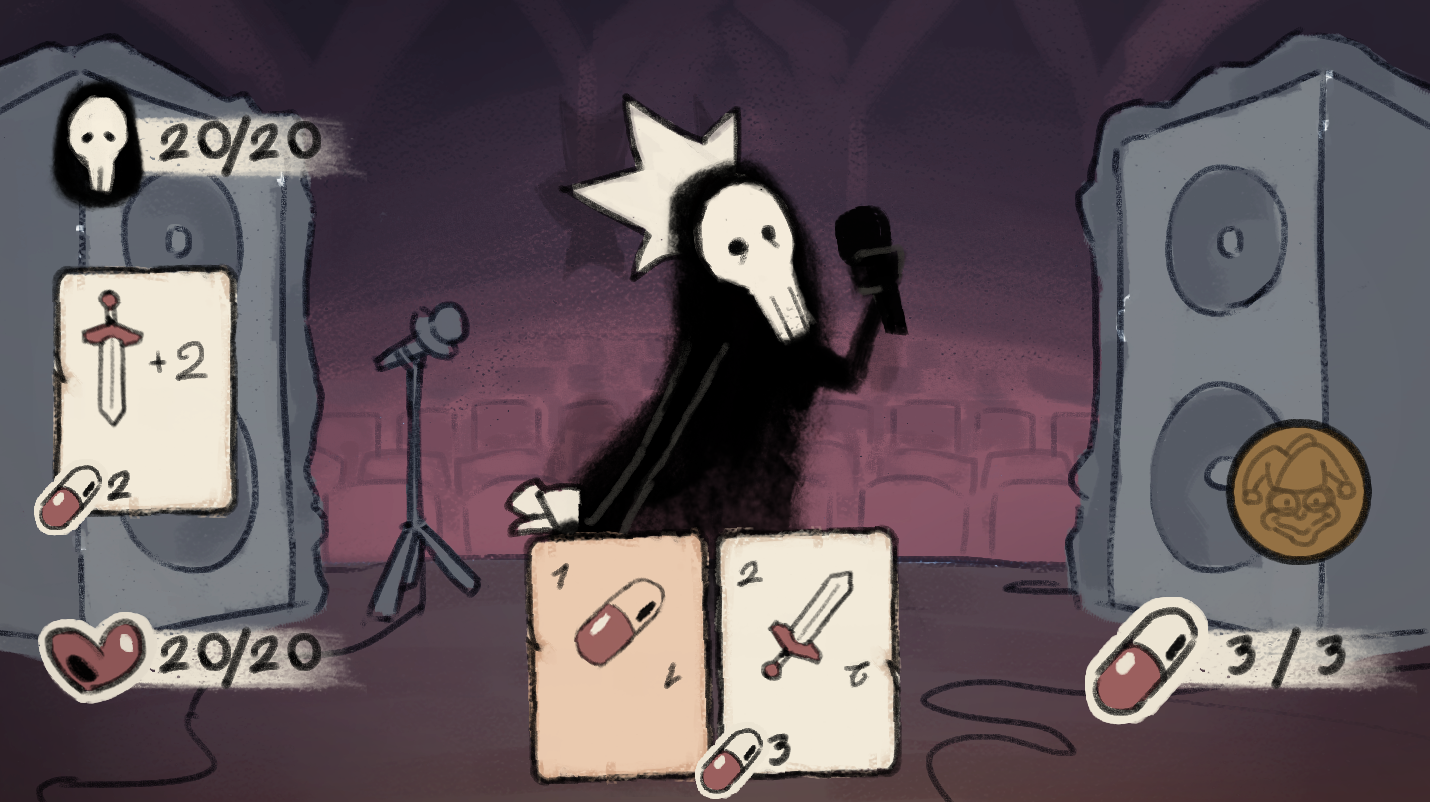
\includegraphics[width=0.9\textwidth]{encore.png}
    \caption{Image from the GameJam's Itch.io~[citation]}
    \label{fig:encore-picture}
    Encore! developed during the 2024 GameJam by Belonzik and TheMultiplexx is a dueling card game with outstanding attention to detail, exploring the theme of death. It stands out for its excellent graphics, well-crafted audio, immersive story, and even professional-grade narration.
\end{figure}

\begin{figure}[H]
    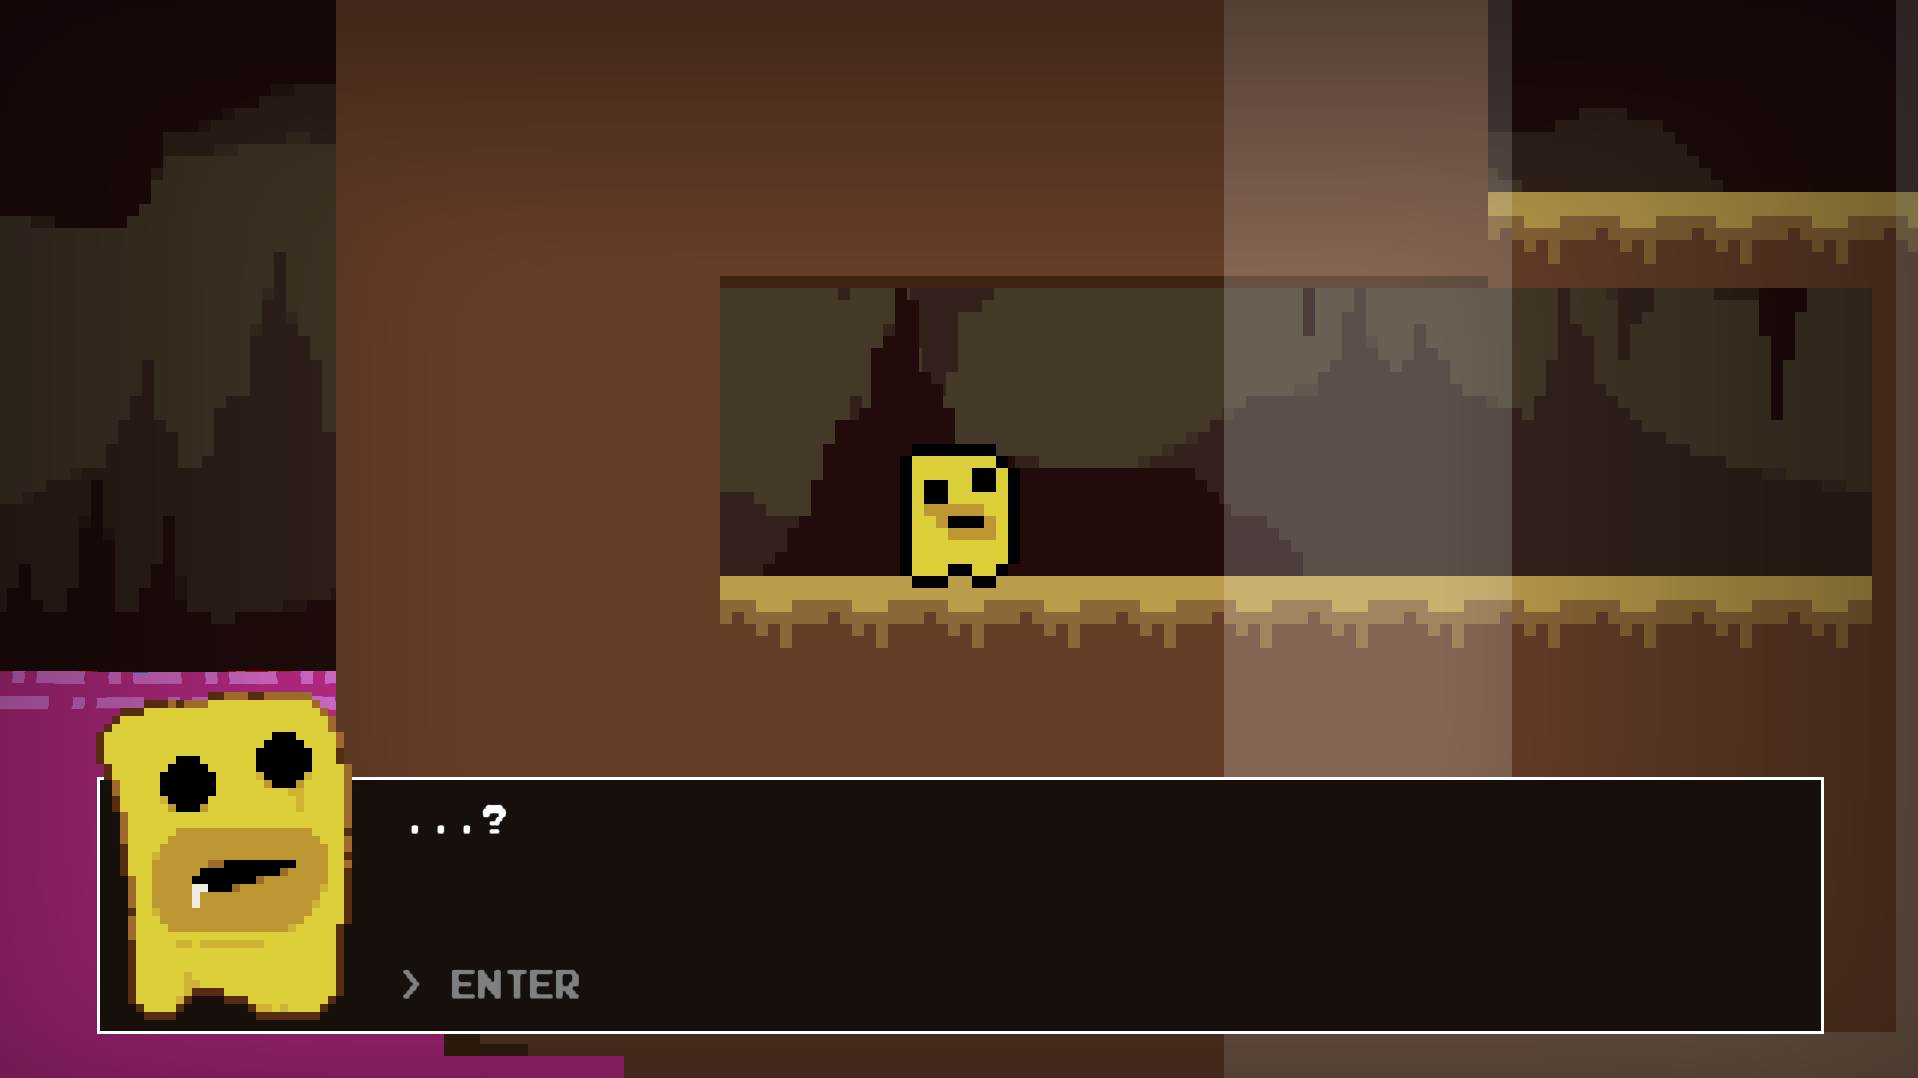
\includegraphics[width=0.9\textwidth]{liminal.png}
    \caption{Image from the GameJam's Itch.io~[citation]}
    \label{fig:liminal-picture}
    Liminal! by HyperCubic Studio was developed during the 2024 GameJam too. This short platform puzzle game traps the player in a twisted TV show. The game’s colourful visuals are beautiful, cohesive and extensively polished. It boasts original mechanics and is full of details in the sounds, menu items and dialogue.
\end{figure}

\begin{figure}[H]
    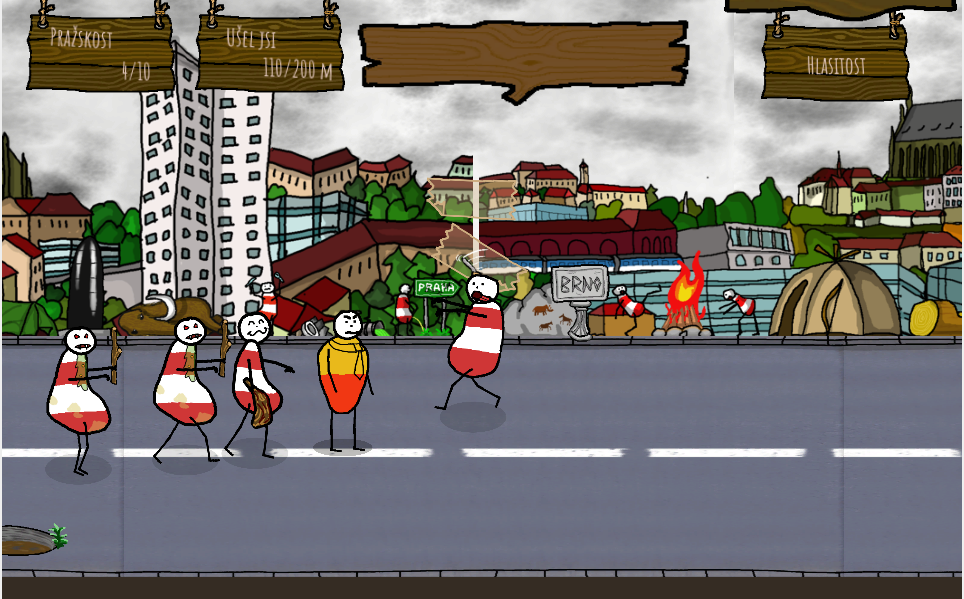
\includegraphics[width=0.9\textwidth]{brno.png}
    \caption{Image from the GameJam's Itch.io~[citation]}
    \label{fig:brno-picture}
    Escape from Brno was created during the 2022 GameJam by Trampod, SharpFoxDev, benjaminhejl, leia12321 and VAHAnima. This side-scrolling dodger won the popular vote among the participants. Its humorous sound design, cohesive graphics, and intuitive gameplay make it feel natural and engaging.
\end{figure}

\begin{figure}[H]
    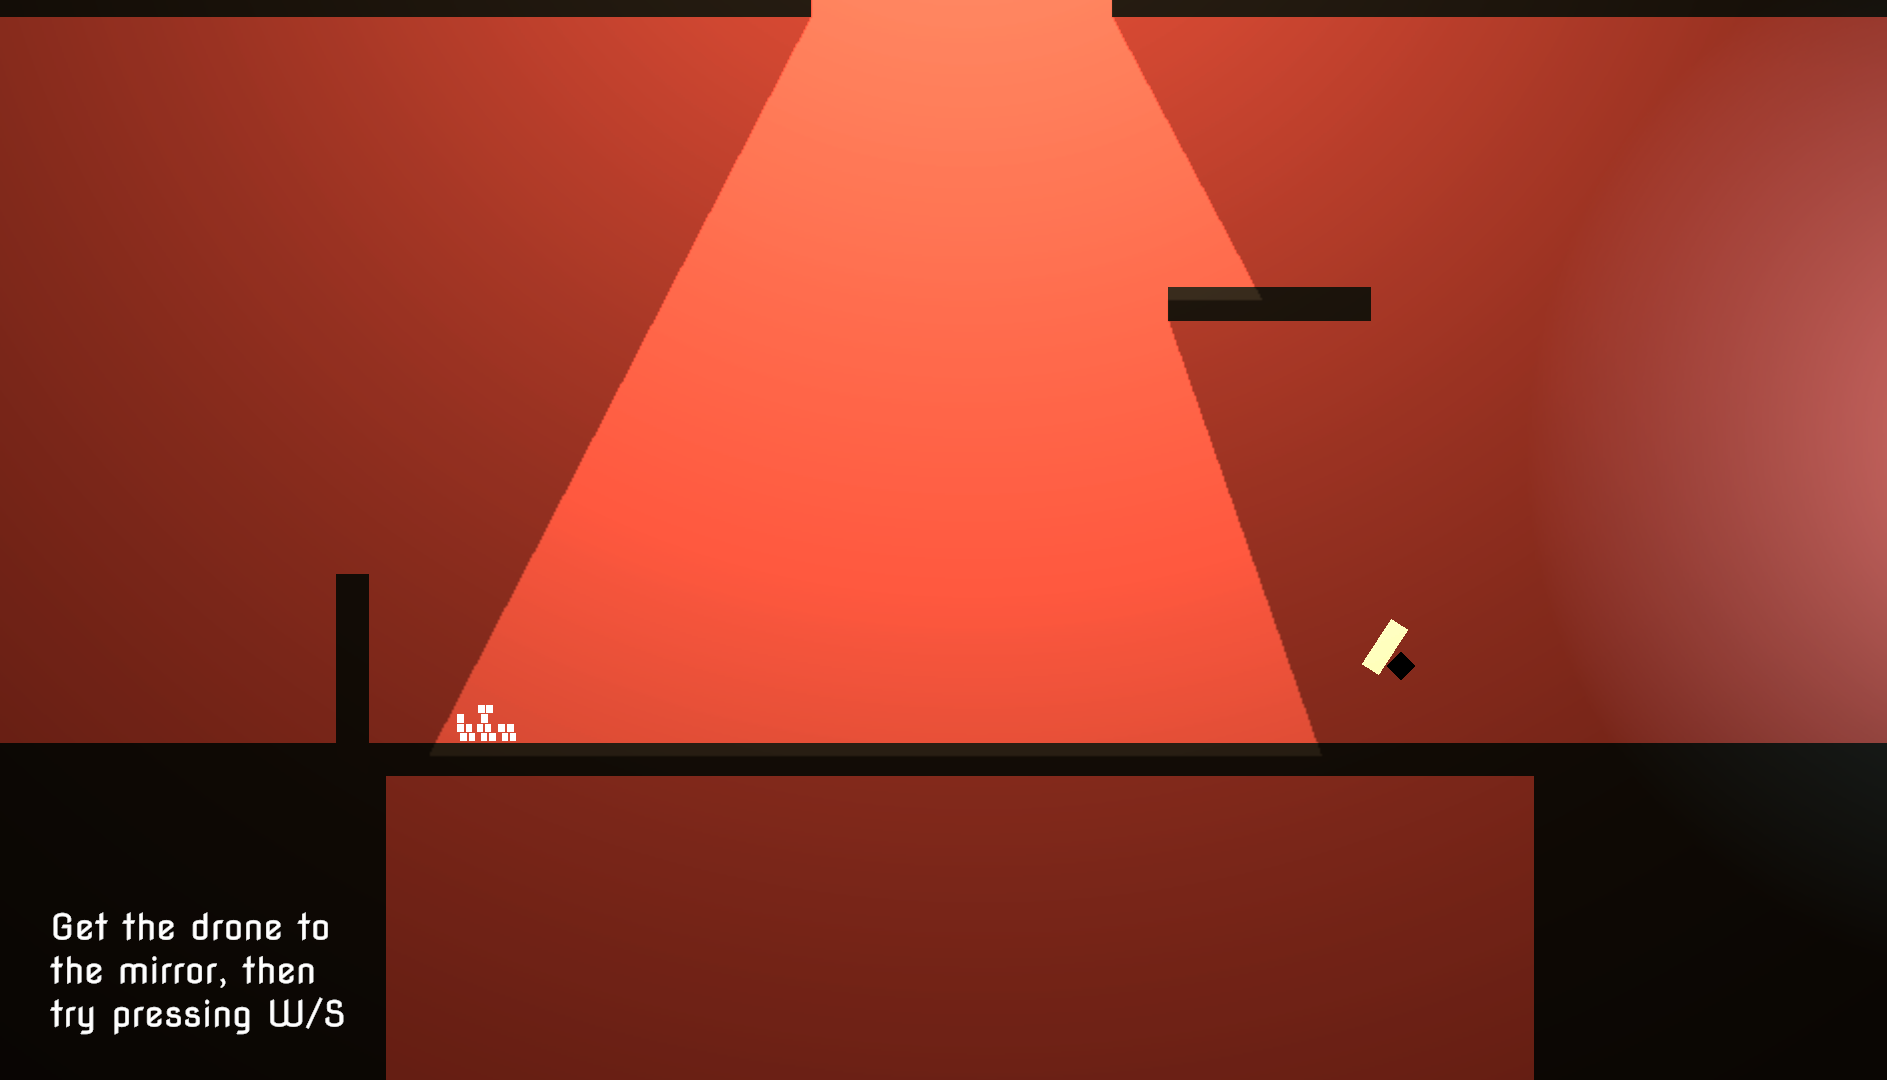
\includegraphics[width=0.9\textwidth]{subject.png}
    \caption{Image from the GameJam's Itch.io~[citation]}
    \label{fig:subject-picture}
    Subject 42 was created by LukyDrum during the 2023 GameHack. This game puts the player in control of a robot’s AI as they solve puzzles and navigate three intriguing levels. A fitting sound-track and a voice sarcastically commenting on the player’s performance contribute to its unique style and storytelling.
\end{figure}

%===============================================================
\section{Local Student Entrepreneurship Support}
While FIT CTU does not currently provide entrepreneurial support, it does facilitate cooperation with industry partners and manages grants for research labs. The university takes over the responsibility of arranging access to dedicated incubators and coaching centers. These initiatives help students refine their business ideas and develop their skills.

One such initiative is InQbay, a CTU-wide programme supporting student, phd, and faculty entrepreneurs. It offers individual coaching, workshops, tutorials, networking events, and access to legal, tax, and marketing consultants.

In addition, the CTU career centre offers an eight-week long entrepreneurship course. It covers ideation, market research, business plan creating, pitching a project, gathering feedback and seeking mentors or investors.
